\tikzset{every picture/.style={line width=0.75pt}} %set default line width to 0.75pt        

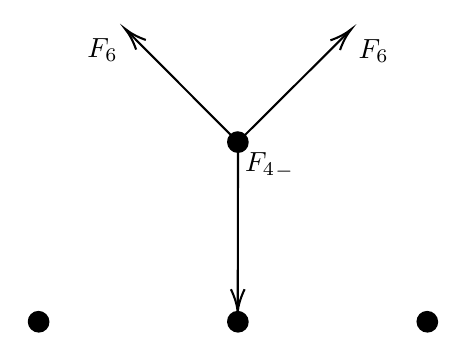
\begin{tikzpicture}[x=0.75pt,y=0.75pt,yscale=-1,xscale=1]
%uncomment if require: \path (0,300); %set diagram left start at 0, and has height of 300

%Shape: Circle [id:dp8570105127026377] 
\draw  [color={rgb, 255:red, 0; green, 0; blue, 0 }  ,draw opacity=1 ][fill={rgb, 255:red, 0; green, 0; blue, 0 }  ,fill opacity=1 ] (322.65,81.72) .. controls (322.6,79.11) and (324.68,77) .. (327.29,77) .. controls (329.9,77) and (332.05,79.11) .. (332.09,81.72) .. controls (332.14,84.33) and (330.06,86.45) .. (327.45,86.45) .. controls (324.84,86.45) and (322.69,84.33) .. (322.65,81.72) -- cycle ;
%Shape: Circle [id:dp4245007933940925] 
\draw  [color={rgb, 255:red, 0; green, 0; blue, 0 }  ,draw opacity=1 ][fill={rgb, 255:red, 0; green, 0; blue, 0 }  ,fill opacity=1 ] (322.65,168.28) .. controls (322.6,165.67) and (324.68,163.55) .. (327.29,163.55) .. controls (329.9,163.55) and (332.05,165.67) .. (332.09,168.28) .. controls (332.14,170.89) and (330.06,173) .. (327.45,173) .. controls (324.84,173) and (322.69,170.89) .. (322.65,168.28) -- cycle ;
%Shape: Circle [id:dp10932705047210622] 
\draw  [color={rgb, 255:red, 0; green, 0; blue, 0 }  ,draw opacity=1 ][fill={rgb, 255:red, 0; green, 0; blue, 0 }  ,fill opacity=1 ] (413.92,168.28) .. controls (413.88,165.67) and (415.95,163.55) .. (418.56,163.55) .. controls (421.17,163.55) and (423.32,165.67) .. (423.37,168.28) .. controls (423.42,170.89) and (421.34,173) .. (418.73,173) .. controls (416.12,173) and (413.97,170.89) .. (413.92,168.28) -- cycle ;
%Shape: Circle [id:dp13666466165408409] 
\draw  [color={rgb, 255:red, 0; green, 0; blue, 0 }  ,draw opacity=1 ][fill={rgb, 255:red, 0; green, 0; blue, 0 }  ,fill opacity=1 ] (236.09,168.28) .. controls (236.14,170.89) and (234.06,173) .. (231.45,173) .. controls (228.84,173) and (226.69,170.89) .. (226.65,168.28) .. controls (226.6,165.67) and (228.68,163.55) .. (231.29,163.55) .. controls (233.9,163.55) and (236.05,165.67) .. (236.09,168.28) -- cycle ;
%Shape: Boxed Line [id:dp4412401484637065] 
\draw    (327.45,86.45) -- (327.29,161.55) ;
\draw [shift={(327.29,163.55)}, rotate = 270.12] [color={rgb, 255:red, 0; green, 0; blue, 0 }  ][line width=0.75]    (10.93,-3.29) .. controls (6.95,-1.4) and (3.31,-0.3) .. (0,0) .. controls (3.31,0.3) and (6.95,1.4) .. (10.93,3.29)   ;
%Shape: Boxed Line [id:dp899763866751071] 
\draw    (327.37,81.72) -- (274.38,28.5) ;
\draw [shift={(272.97,27.09)}, rotate = 405.12] [color={rgb, 255:red, 0; green, 0; blue, 0 }  ][line width=0.75]    (10.93,-3.29) .. controls (6.95,-1.4) and (3.31,-0.3) .. (0,0) .. controls (3.31,0.3) and (6.95,1.4) .. (10.93,3.29)   ;
%Shape: Boxed Line [id:dp6686588216420633] 
\draw    (327.37,81.72) -- (380.59,28.73) ;
\draw [shift={(382.01,27.32)}, rotate = 495.12] [color={rgb, 255:red, 0; green, 0; blue, 0 }  ][line width=0.75]    (10.93,-3.29) .. controls (6.95,-1.4) and (3.31,-0.3) .. (0,0) .. controls (3.31,0.3) and (6.95,1.4) .. (10.93,3.29)   ;

% Text Node
\draw (270.97,30.49) node [anchor=north east] [inner sep=0.75pt]    {$F_{6}$};
% Text Node
\draw (384.01,30.72) node [anchor=north west][inner sep=0.75pt]    {$F_{6}$};
% Text Node
\draw (329.37,85.12) node [anchor=north west][inner sep=0.75pt]    {${F_{4}}_{-}$};


\end{tikzpicture}
